%%%%%%%%%%%%%%%%%%
%%% Chapitre 2 %%%
%%%%%%%%%%%%%%%%%%
\chapter{Un premier projet à l'aide d'un \textit{IDE}}
Tout projet \textit{Python} possède la même structure commune de base:
\begin{verbatim}
    - Répertoire (nom du projet)
          |
          |
          ---- Fichier principal (main.py)
\end{verbatim}
\medskip

Plus le projet est important, plus il contiendra de sous répertoires et fichiers (nous verrons cela en temps voulu).
\medskip

\section{Avec \textit{Pycharm}}
Au lancement de \textit{Pycharm} on sélectionne \texttt{New Project}.
\begin{figure}[h]
\begin{center}
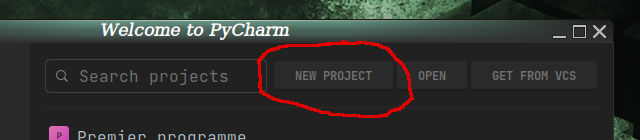
\includegraphics[scale=0.3]{IMG/Pycharm-01.png}
\caption{Nouveau projet avec \textit{Pycharm}}
\end{center}
\end{figure}
\medskip

Puis dans la fenêtre qui s'ouvre on va spécifier le répertoire du projet (\texttt{Location}) et l'interpréteur \textit{Python} que l'on va utiliser (\texttt{Base interpreter}). Ensuite, cliquer sur \texttt{Create}. Pour le reste on ne s'en occupe pas pour le moment.
\begin{figure}[h]
\begin{center}
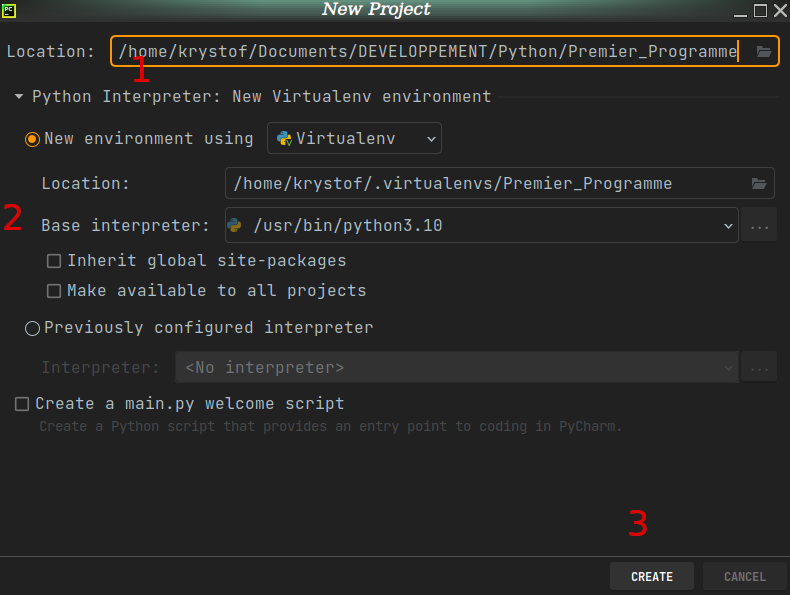
\includegraphics[scale=0.25]{IMG/Pycharm-02.png}
\caption{Création du projet avec \textit{Pycharm}}
\end{center}
\end{figure}
\medskip

Pour créer le premier fichier (notre \texttt{main.py}), faire un clic droit sur le nom du projet qui se situe dans le panneau de gauche (panneau \textit{project}). Sélectionner:
\begin{verbatim}
    New > Python File
\end{verbatim} 
Et nommer ce fichier \texttt{main}.
\begin{figure}[h]
\begin{center}
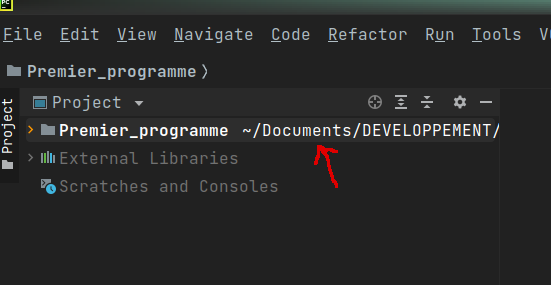
\includegraphics[scale=0.5]{IMG/Pycharm-03.png}
\caption{Premier fichier d'un projet avec \textit{Pycharm}}
\end{center}
\end{figure}
\medskip

Pour illustrer l'exécution du code avec \textit{Pycharm} nous allons tout d'abord insérer la ligne suivante dans le fichier \texttt{main.py}\footnote{\texttt{print()} est une fonction et \texttt{"Bonjour"} son paramètre.}:
\begin{verbatim}
    print("Bonjour")
\end{verbatim}
\medskip

La première fois que l'on lance un programme avec \textit{Pycharm} il faut faire un clic droit sur le panneau de l'éditeur, sélectionner dans le menu déroulant qui s'affiche \texttt{Run "main"}. Cette première fois permet à \textit{Pycharm} de créer une configuration que nous pourrons alors utiliser pour les prochaines exécutions du code, à l'aide du bouton \texttt{Run} en haut à gauche de l'\textit{IDE}.
\begin{figure}[h]
\begin{center}
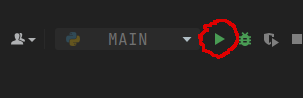
\includegraphics[scale=0.5]{IMG/Pycharm-04.png}
\caption{Lancement du programme avec la touche \texttt{Run}.}
\end{center}
\end{figure}
\medskip

S'ouvre alors le panneau d'exécution du code (panneau \textit{Run}) en bas de l'interface \textit{Pycharm} dans lequel on voit le résultat de notre programme précédé d'une ligne du type:
\begin{verbatim}
    ~/.virtualenvs/Premier_programme/bin/python  ~/Premier_
    programme/main.py
\end{verbatim}
\verb|~/.virtualenvs/Premier_programme/bin/python| représente l'interpréteur auquel nous faisons appel et \verb|~/Premier_programme/main.py| le fichier du code qui sera exécuté.
medskip

\section{Avec \textit{Visual Studio Code}}
Avec \textit{VSC} nous ne sommes pas obligés d'en passer par la création d'un projet. Si le projet ne doit contenir qu'un unique fichier, il peut être en effet plus simple et plus léger d'en passer par cet \textit{IDE}. Pour cela:
\begin{verbatim}
    Fichier > Nouveau fichier > Enregistrer sous
\end{verbatim}
On doit alors choisir le répertoire et donner un nom au fichier qui doit porter l'extension \texttt{.py}.
\medskip

\section{L'exécution du code}
Dans un programme la lecture des lignes de code est séquentielle, un ordre est donc suivi. 
\medskip

Maintenant que nous avons notre premier fichier, nous allons pouvoir entrer dans le coeur du langage \textit{Python} en commençant par aborder les concepts de base.
\medskip
